\chapter{Deseño e implementación}
\label{cap:design}
\minitoc
% \label{chap:Desenoeimplementacion}
% \vspace{0.5cm}

%%%%%%%%%%%%%%%%%%%%%%%%%%%%%%%%%%%%%%%%%%%%%%%%%%%%%%%%%%%%%%%%%%%%%%%%%%%%%%%%
% Objetivo:                        %
%%%%%%%%%%%%%%%%%%%%%%%%%%%%%%%%%%%%%%%%%%%%%%%%%%%%%%%%%%%%%%%%%%%%%%%%%%%%%%%%

  \lettrine{N}{este} capítulo veremos os detalles de deseño e implementación 
de diversas partes do proxecto e falaremos das decisións tomadas con 
respecto a utilización das múltiples tecnoloxías utilizadas.

  Comezaremos facendo unha pequena introducción á terminoloxía e ás tecnoloxías 
utilizadas no proxecto na Sección~\ref{sec:design:react}, xa que resulta 
fundamental para comprender as diversas explicacións técnicas sobre o deseño e 
a implementación.

  Falaremos tamén das bases de datos non relacionais na 
Sección~\ref{sec:design:db}, comentaremos a necesidade da creación da 
aplicación como App híbrida e todo isto seguido dunha extensa análise sobre a 
usabilidade e as múltiples decisións que se tomaron ao respecto, debido a gran 
importancia que ten este campo dentro do proxecto.

  Por último tamén comentaremos algún conflito que xurdíu durante o 
desenvolvemento a nivel de dependencias de paquetes ou testing e as decisións 
que se tomaron para solventalos.

  \section{ReactJS e Flux}
  \label{sec:design:react}
    \subsection{Introdución e elección da tecnoloxía}
    Actualmente o mundo das aplicacións móbiles está en pleno crecemento e cada 
vez é máis sinxelo ver cómo pequenos comercios ou incluso eventos de ocio 
como festivais de música ou conferencias, teñen a súa propia aplicación 
móbil\footnote{Eventos como o FOSDEM, a LibreCon ou OpenExpo xa dispoñen de 
aplicacións móbiles para facilitar os asistentes organicen as actividades ás 
que asistirán.}.

    A sociedade está a eliminar un soporte tradicional como é o papel, en 
tódolos aspectos da vida, dende a publicidade ata a propia xestión do traballo, 
e todo estase a dixitalizar, facilitando o traballo humano e reducindo os custes 
a medio prazo.

    Neste contexto decidíuse optar por realizar unha aplicación móbil 
híbrida, con tecnoloxías web, xa que se pode observar un movemento nos últimos 
anos cara este tipo de tecnoloxías que permiten desenvolver únicamente unha 
aplicación e executala nos diversos sistemas operativos móbiles existentes, sen 
ter que desenvolver unha aplicación concreta para cada un de eles.

    Tras unha análise das diversas linguaxes e frameworks que podían 
ser utilizados para este fin, finalmente optouse por utilizar ReactJS pola sua 
flexibilidade fronte a outras alternativas como AngularJS ou EmberJS.

    Estas alternativas céntranse en ofrecer un framework moi completo buscando 
cubrir todos os aspectos de unha aplicación como o enrutado 
de urls, a internacionalización ou os servizos, fronte a React que únicamente 
trata de cubrir a xestión das vistas e do seu estado, dando total liberdade 
para escoller a tecnoloxía que se precise para o resto de compoñentes da 
aplicación.

    Así mesmo tamén cómpre destacar a existencia de React Native, unha 
tecnoloxía baseada en React que permite crear aplicacións móbiles con 
tecnoloxías web e con unha experiencia de usuario exactamente igual a unha 
aplicación nativa tradicional.

    Unha vez selecciado React, optamos por seguir a arquitectura máis habitual 
dentro de este tipo de aplicacións, Flux, a través da librería Reflux.

    \subsection{Elementos básicos}
      \subsubsection{Compoñentes de React}
      React é unha librería de Javascript que nos permite xestionar de xeito 
sinxelo as vistas da nosa aplicación a través de diversos elementos denominados 
compoñentes.

      React permítenos escribir os nosos compoñentes con unha sintaxis moi 
similiar a HTML pero posteriormente traduce esta sintaxis a código javascript 
habitual polo que podemos decir que estamos escribindo páxinas web únicamente 
con funcións de javascript.

      A idea principal é reutilizar e agrupar compoñentes para formar o que 
tradicionalmente chamamos vistas e que a súa vez poden ter un estado.
      Este estado pode variar modificando as vistas, como por exemplo cando se 
engade un novo gol na lista de eventos e React encárgase de volver a 
renderizar únicamente a parte da vista que cambiou, polo que é tremendamente 
eficiente.

      \subsubsection{Arquitectura Flux}
      Flux\cite{book:flux} é unha arquitectura que básicamente propón o esquema 
mostrado na Figura~\ref{fig:img:flux}.

        \begin{figure}[h!]
          \begin{center}
          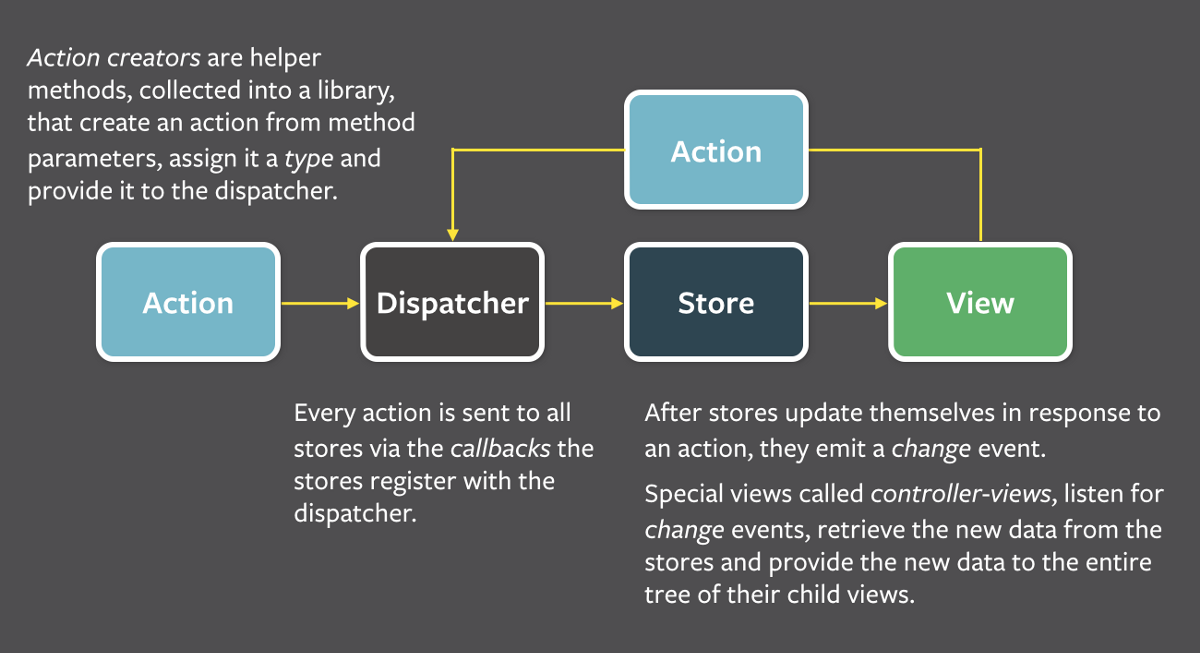
\includegraphics[width=\textwidth]{./img/flux.png}
          \caption{Esquema da arquitectura Flux}
          \label{fig:img:flux}
          \end{center}
        \end{figure}

      Unha aplicación que opte por seguir esta arquitectura debe conter os 
seguintes compoñentes:

        \paragraph{Actions}
        A vista atópase formada por unha serie de compoñentes de React que son 
capaces de disparar as Actions, por exemplo ao pulsar un botón, e que funcionan 
de xeito similar a eventos, notificando ao Dispatcher cando se produce a súa 
execución.
        \paragraph{Dispatcher}
        O Dispatcher é o encargado de recibir e enrutar as Actions disparadas 
cara as Stores.
        \paragraph{Stores}
        Estas Stores son as encargadas de xestionar o estado dos compoñentes e 
toda a lóxica necesaria para actualizar o estado co novo cambio.

        Se por exemplo ao pulsar un botón debería cambiar un texto que está no 
compoñente, poderíamos ter este texto almacenado no estado dentro dunha Store e 
inicializado a un valor baleiro.
        Unha vez se fai click no botón, unha Action chamará a unha Store que é 
a que contén a información sobre cómo cambiar o texto do estado e React 
encargarase de volver a pintar o novo valor do estado, dentro do seu compoñente.

      \subsubsection{Implementación de Flux. Reflux.}
      Flux é unha arquitectura, unha especie de patrón de desenvolvemento pero 
existen diversas implementacións da mesma e neste proxecto decidímonos por 
utilizar Reflux\cite{web:reflux}.

      O funcionamento é moi similar pero con algúns matices; por exemplo,
non existe un único Dispatcher central que enruta as Actions se non que todas as 
Stores están escoitando e reaccionan cando teñen un método para responder a 
Action.

     Vexamos un exemplo práctico:

    \lstset{}
     \begin{lstlisting}[caption=Exemplo de Action., label=fig:design:action]
let TextActions = Reflux.createActions([
  "updateText"
])
    \end{lstlisting}

    Definiríamos unha Action (Fragmento de código~\ref{fig:design:action}). que 
queremos lanzar para tratar de actualizar o texto e crearíamos unha Store 
(Fragmento de código~\ref{fig:design:store}) que escoite as TextActions e que 
implemente unha función onUpdateText que será a que reciba o novo valor e 
actualizará o estado.

    \lstset{}
     \begin{lstlisting}[caption=Exemplo de Store., label=fig:design:store]
let TextStore = Reflux.createStore({
  listenables: TextActions,
  init: function () {
    this.state = ''
  },
  getInitialState: function () {
    return this.state
  },
  onUpdateText: function (newText) {
    this.state = newText
    this.trigger(this.state)
  }
})
    \end{lstlisting}

    Por último definir o compoñente (Fragmento de 
código~\ref{fig:design:component}). Este deberá incluir unha lista de mixins 
onde indicarlle cales son as Stores que reaccionan ante eventos lanzados 
dende este compoñente, neste caso, a TextStore.

    O compoñente tamén terá un método render no que definir o que poderíamos 
chamar informalmente a ``vista'' do que queremos renderizar, e que inclúe un 
enlace para cambiar o texto mostrado.

    Dito enlace reacciona cando se fai click e chama ao método 
handleChangeTextClick que lanza a Action para que a Store a intercepte, cambie 
o estado e React renderice de novo, únicamente o que cambiou.

    \lstset{}
     \begin{lstlisting}[caption=Exemplo de compoñente de React., 
label=fig:design:component]
let EndReport = React.createClass({
  mixins: [
    Reflux.connect(TextStore, 'text')
  ],
  handleChangeTextClick: function () {
    TextActions.updateText('Nuevo texto a renderizar')
  }
render: function () {
    return (
      <p>{this.state}</p>
      <a onClick={this.handleChangeTextClick}>Change text</a>
    )
  }
})
    \end{lstlisting}


    \subsection{Estructura da aplicación}

    A continuación móstranse os diversos elementos xerais que contén a 
aplicación, as carpetas principais e certos ficheiros fundamentais na execución 
da aplicación.

      \begin{description}
        \item [tests] Carpeta onde se poden atopar os tests da aplicación. De 
momento só se dispón de tests da capa de servizos.
        \item [i18n] Nesta localización pódese atopar a internacionalización, 
coas cadeas dentro da subcarpeta de ``messages`` e coa descrición das mesmas 
para cada compoñente de React dentro de ''descriptors``, coa idea de darlle 
contexto e facilitarlle ao tradutor a súa labor.
        \item [cordova app] Aquí podemos atopar a configuración para compilar a 
aplicación aos diversos dispositivos móbiles.
        \item [src/app] Estrutura principal da aplicación
        \begin{description}
          \item [Actions] Lista de ficheiros con accións a disparar, agrupados 
cada un pola store que o implementa.
          \item [API] Contén a configuración, as urls da aplicación e a 
factoría utilizada para a inxección de dependencias dos servizos que 
explicaremos máis adiante.
          \item [Components] Lugar onde se poden atopar todos os compoñentes 
que forman as vistas da aplicación. 
          \item [Daos] Entidades que abstraen dos servicios a definición do 
acceso a base de datos, facilitando que sexa sinxelo cambiar dita base de datos 
se é preciso.
          \item [Models] Contén a definición dos modelos da aplicación, tanto as 
entidades que se almacenan en base de datos como de certas clases que son 
utilizadas pola aplicación, como por exemplo as que definen os deportes ou a 
implementación dos tipos de eventos.
          \item [Services] Estas clases conteñen a lóxica de negocio da 
aplicación.
          \item [Stores] Lista de ficheiros que conteñen e xestionan o estado da 
aplicación. Cómpre diferenciar a lóxica de negocio, que se almacena nos 
servizos, da xestión do estado dos compoñentes de React que podemos atopar nas 
Stores.
          \item [app.js] Ficheiro de inicialización da aplicación que se encarga 
de arrancar o enrutador e executa a aplicación ben en modo web ou ben en modo 
aplicación móbil en función da configuración definida.
          \item [router.jsx] É o encargado de poñer en relación as urls da 
aplicación cos compoñentes que corresponden a cada unha e onde se introduce 
tamén, a información sobre a internacionalización.

        \end{description}

      \end{description}


  \section{Bases de datos e funcionamento offline}
  \label{sec:design:db}
  O mundo das bases de datos está a cambiar enormemente nos últimos anos coa 
aparición das bases de datos non relacionais\cite{book:nosql}, neste caso 
concreto, era preciso 
dispoñer de unha base de datos no cliente que permitise almacenar os 
datos das actas dos encontros de forma offline xa que o árbitro do encontro, 
pode non ter cobertura e debería poder cubrir a súa acta da mesma forma.

  Ante este requisito cabe pensar en bases de datos lixeiras como SQLite que 
se utilizan habitualmente nas aplicacións móbiles pero ditas bases de datos non 
poden ser executadas directamente nun navegador web, polo que finalmente se 
optou por utilizar PouchDB, unha base de datos orientada a documentos e creada 
sobre o GlobalStorage\footnote{Un obxecto que mantén múltiples áreas de 
almacenamento privado para almacenar datos durante un largo periodo de tempo} 
do navegador, pensada dende o primeiro momento para crear aplicacións web que 
funcionen de forma desconectada.

    \subsection{PouchDB}
    As actas electrónicas son documentos que unha vez sexan creadas, apenas 
serán modificadas e neste tipo de información, son as bases de datos orientadas 
a documentos as que presentan un mellor rendemento.

    A elección de PouchDB\cite{web:pouchdb} foi sobre todo motivada por ser 
tremendamente lixeira, multinavegador e sobre todo, facilitar a sincronización 
contra unha base de datos remota, neste caso, CouchDB.

    \subsection{CouchDB}
    CouchDB\cite{web:couchdb} é a base de datos non relacional que se utiliza 
como base de datos central en remoto, e coa cal sincronizará PouchDB que se 
atopa no navegador web do cliente.

    Esta base de datos é tremendamente versatil e sinxela de utilizar xa que 
implementa unha API REST e, a forma de interactuar con ela basease simplemente 
en enviar documentos JSON a través de sinxelas peticións HTTP cara a súa API.

    Destaca pola súa extensa comunidade e por ser altamente dispoñible e 
tolerante a erros pero eventualmente inconsistente, aínda que foi crítico na 
súa elección a xestión que CouchDB fai dos conflictos de datos e que comentamos 
a continuación

    \subsection{Sincronización e xestión de conflictos}
    Probablemente o maior reto á hora de enfrentarse a unha aplicación con 
funcionamento offline é a xestión de conflictos entre os datos.

    En este caso en concreto, existe a problemática de que por múltiples 
motivos, un acta pode ser modificada en dous lugares ao mesmo tempo, tanto polo 
árbitro no seu teléfono como pola persoa encargada da xestión da federación
polo que resulta imprescindible non perder información e ser capaces de 
mostrarlle a totalidade da información ao xestor da federación para que este 
poida seleccionar cales datos son os reais.

    Neste punto é donde CouchDB resulta moi útil xa que a propia base de datos 
se encarga de almacenar unha árbore co histórico de revisións que se producen 
sobre un documento e así se poderían mostrar ao usuario para que seleccione a 
correcta en caso de conflicto.

  \section{App híbrida con Apache Cordova}
  O obxectivo do proxecto é poder utilizalo en múltiples dispositivos móbiles 
co fin de facilitar que calquera árbitro poida utilizala independentemente do 
sistema operativo que teña o seu teléfono ou tableta.

  É por isto que é fundamental a utilización dun sistema que permita este 
desenvolvemento multiplataforma como é o caso de Apache 
Cordova\cite{web:apachecordova} que, ademáis, 
facilita o acceso aos elementos do dispositivo como sensores, datos, estado de 
rede... a través dunha serie de APIs estandar.

  Actualmente non se está a utilizar ningunha de estas funcionalidades pero si 
é posible que nun futuro cercano se decidan implementar novas características 
que si precisen o acceso a este tipo de elementos como pode ser por exemplo, o 
micrófono, para que o árbitro poida gardar as incidencias dun partido como 
notas de voz en lugar de escribilas.

  Na Figura~\ref{fig:design:cordova_arquitectura} podemos ver un esquema da 
arquitectura dunha aplicación sobre Apache Córdova.

    \begin{figure}[h!]
      \begin{center}
      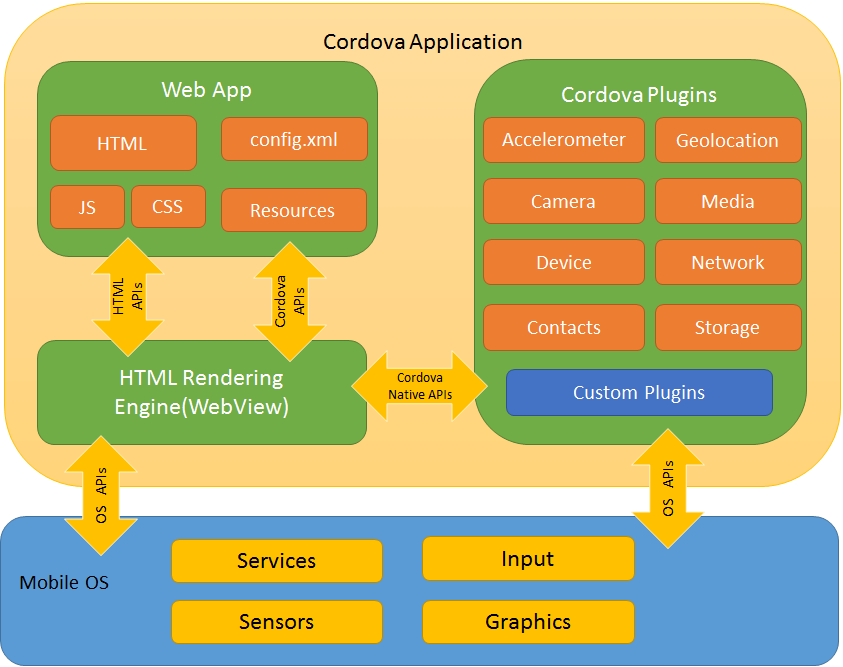
\includegraphics[width=0.8\textwidth]{./img/cordova_arquitectura.png}
      \caption{Arquitectura de unha aplicación con Apache Cordova}
      \label{fig:design:cordova_arquitectura}
      \end{center}
    \end{figure}

  Básicamente a aplicación executase como unha aplicación web normal sobre un 
WebView, un motor de renderizado de HTML que pode interactuar coas APIs nativas 
do dispositivo a través dunha serie de plugins que Cordova provee.

  Para executar a aplicación únicamente é preciso crear un proxecto de Cordova, 
engadir os ficheiros da aplicación, as plataformas para as que se desexe xerar 
o proxecto e construilo.
\clearpage
  \section{Interface gráfica e usabilidade}
  A importancia da interface gráfica en este proxecto é crucial, debido a que a 
aplicación será utilizada por persoas de un amplísimo rango de idades, a 
usabilidade é o valor máis importante.

  A nivel de deseño a aplicación separase en catro grandes bloques:

  \todo{Engadir gráfico}
  \begin{figure}[h!]
    \begin{center}
    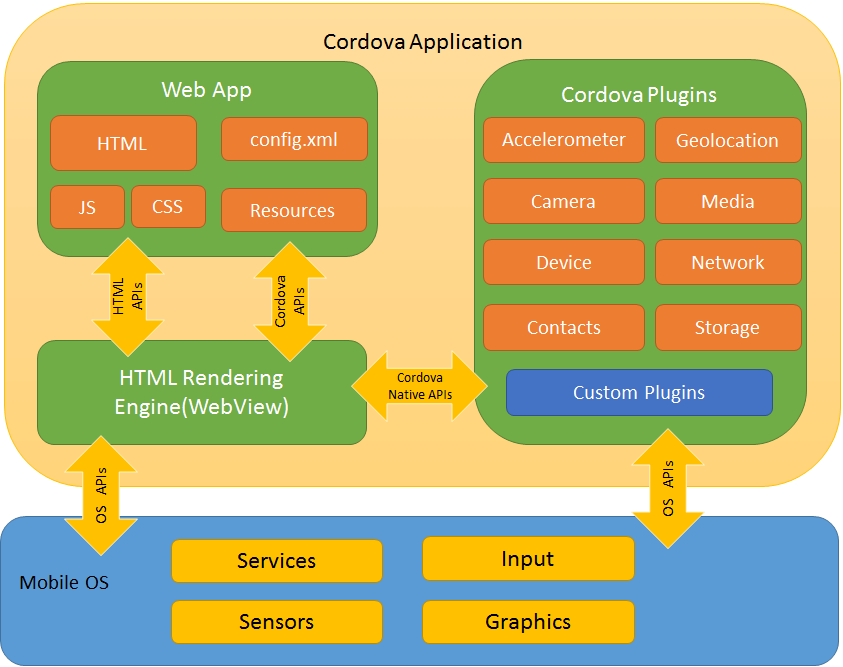
\includegraphics[width=0.2\textwidth]{./img/cordova_arquitectura.png}
    \caption{Estructura da aplicación gráficamente.}
    \end{center}
  \end{figure}

    \subsection{Elementos comúns}
    Para facilitar o desenvolvemento da aplicación creáronse varios 
compoñentes de React xenéricos que permiten realizar tarefas comúns a múltiples 
partes da aplicación, e polo tanto, que son utilizados dende outros compoñentes 
de React.

      \subsubsection{Menú lateral esquerdo}
      É o menú principal da aplicación e que se mostra ao pulsar no botón 
superior esquerdo dende a maior parte de vistas.

      Como se pode ver na Figura~\ref{fig:design:leftmenu}, este 
menú desplegable mostra actualmente o logotipo de VACmatch e unha 
serie de enlaces entre os que se atopan as páxinas de configuración e a páxina 
''acerca de``.

      Para xestionar os enlaces que se mostran en cada páxina de forma 
internacionalizada, e para permitir dispoñer dos elementos nun sitio 
centralizado, creouse o compoñente \lstinline{LeftMenuItems}.
      Este compoñente contén varias listas con items para introducir dentro do 
menú lateral esquerdo e que se poden editar ou engadir outras se é 
preciso.

      Utilizase tamén a MenuStore para xestionar os elementos que 
se atopan actualmente no menú e pódese utilizar a Action 
\lstinline{setLeftMenu} para modificar os elementos que o compoñen en calquera 
momento, por exemplo, ao 
entrar en unha nova vista.

      \begin{figure}[h!]
        \begin{center}
        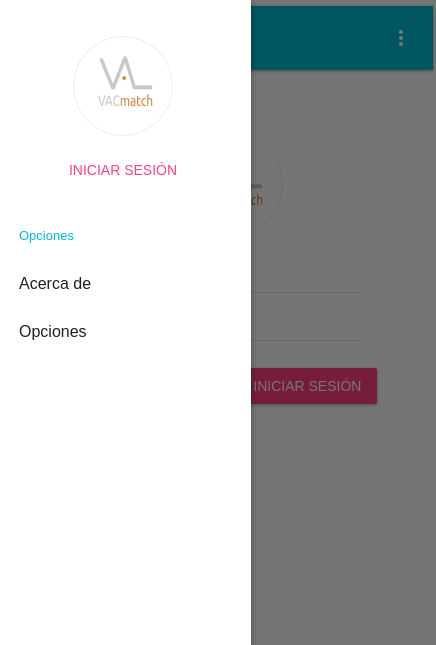
\includegraphics[width=0.5\textwidth]{./img/demo/1_left_menu.png}
        \caption{Menú lateral esquerdo.}
        \label{fig:design:leftmenu}
        \end{center}
      \end{figure}

      \subsubsection{Enlaces do menu superior dereito}
      O funcionamento de este menú é moi similar ao anterior só que este 
non dispón de compoñente propio e únicamente é preciso chamar a Action 
\lstinline{setRightMenu} para colocar a listaxe cos novos elementos a mostrar 
no menú desplegable como se ve na Figura~\ref{fig:design:rightmenu}

      A función debe recibir unha lista de obxectos que conterán os 
seguintes atributos:

      \begin{description}
       \item [text] Texto a mostrar polo item.
       \item [url] Url a onde ir ao facer click no elemento.
       \item [callback] Función de callback que se executará unha vez se 
redirixa a aplicación á url indicada (Opcional).
      \end{description}

      \begin{figure}[h!]
        \begin{center}
        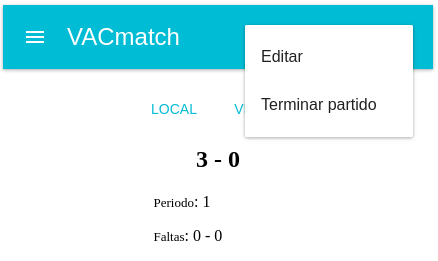
\includegraphics[width=0.5\textwidth]{./img/demo/2_right_menu.png}
        \caption{Menú desplegable dereito.}
        \label{fig:design:rightmenu}
        \end{center}
      \end{figure}


      \subsubsection{Información e axustes}
      Toda aplicación debe conter un apartado de información sobre a mesma, e 
en este caso móstrase ademáis as diversas redes sociais do proxecto e o 
repositorio de código en GitHub para que calquera poida contribuir ao mesmo.

      Por outro lado tamén se ten en conta que toda aplicación debe ser 
personalizable en certa medida, de momento non se dispón de opcións máis ca 
cambiar de idioma pero cando exista a necesidade de incorporar 
novos elementos de configuración, este será o apartado onde os usuarios poderán 
modificar ditas opcións.

      \begin{figure}[h!]
        \begin{center}
        
\includegraphics[width=0.4\textwidth]{./img/demo/3_about.png}
        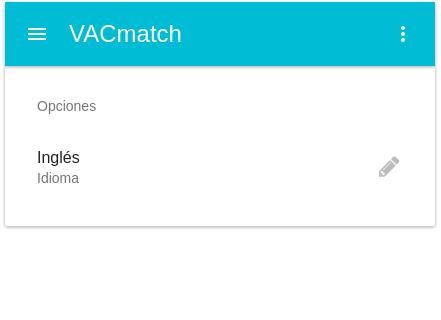
\includegraphics[width=0.4\textwidth]{./img/demo/4_settings.png}
        \caption{Ventás de información e axustes.}
        \label{fig:design:settings}
        \end{center}
      \end{figure}

      \subsubsection{Barra de notificacións}
      Inicialmente xurdíu a necesidade de comunicarlle ao usuario os erros que 
se producen na aplicación, casos concretos como introducir un usuario 
incorrecto ou tratar de eliminar un evento de comezo de partido antes de 
eliminar o de fin do mesmo, deben mostrar un aviso ao usuario.

      É por iso que se decidíu crear unha ``Barra de notificacións'' 
(Figura~\ref{fig:design:notifications}), unha 
pequena ventá que xurde a modo de aviso na parte inferior da pantalla durante 
uns segundos para mostrar información.

      \begin{figure}[h!]
        \begin{center}
        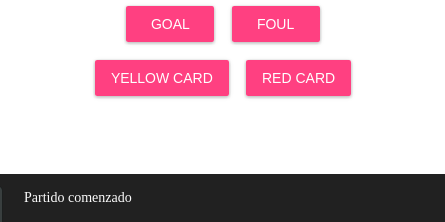
\includegraphics[width=0.5\textwidth]{./img/demo/5_notifications.png}
        \caption{Barra de notificacións.}
        \label{fig:design:notifications}
        \end{center}
      \end{figure}

      Inicialmente pensouse para mostrar os erros pero tamén resulta de 
utilidade a hora de mostrarlle outra información ao usuario como cando un 
evento é engadido correctamente.

      As novas mensaxes son almacenadas na SnackBarStore creada para o caso, 
que permite diferenciar as mensaxes de erro e as de información, facendo que a 
implementación da barra sexa moi sinxela como se mostra no Fragmento de 
código~\ref{fig:design:notificationscode}.

    \lstset{}
      \begin{lstlisting}[caption=Barra de notificacións., 
label=fig:design:notificationscode]
let SnackBarItem = React.createClass({
  mixins: [
    Reflux.connect(SnackBarStore, 'snackBar')
  ],

  onStatusChange: function (status) {
    this.refs.snack.show()
  },

  componentDidMount: function () {
    this.listenTo(SnackBarStore, this.onStatusChange)
  },

  render: function () {
    return <Snackbar key={'generic-snackbar'}
      ref='snack'
      message={this.state.snackBar.message}
      autoHideDuration={4000} />
  }
})

      \end{lstlisting}

      \subsubsection{Autenticación}
      A autenticación é fundamental en esta aplicación xa que únicamente os 
usuarios con acceso poden crear ou modificar actas, neste contexto foi preciso 
crear un compoñente de autenticación que se encargue de realizar a comprobación 
de se o usuario iniciou sesión na aplicación sempre que se carguen os 
compoñentes.

      Creouse unha clase sinxela que deben extender aqueles compoñentes que só 
poidan ser accedidos se o usuario está autenticado, o 
``AuthenticatedComponent'' (Fragmento de código~\ref{fig:design:authcode}) e 
que redirixe a aplicación cara páxina de iniciar sesión, no caso de non poder 
atopar un usuario activo na sesión.

    \lstset{}
    \begin{lstlisting}[caption=Compoñente de autenticación., 
label=fig:design:authcode]
export default (ComposedComponent) => {
  let AuthenticatedComponent = React.createClass({
    mixins: [
      Reflux.connect(AuthStore, 'auth'),
      History
    ],

    componentWillMount: function (transition) {
      if (config._env !== 'development') {
      // This method is called before transitioning to this component.
      // If the user is not logged in, we'll send him or her to the Login page.
        if (!AuthStore.isLoggedIn()) {
          this.history.pushState(null, urls.login.show)
        }
      }
    },

    render: function () {
      return (
        <ComposedComponent
        {...this.props} />
      )
    }
  })
  return AuthenticatedComponent
}
    \end{lstlisting}

    Ao mesmo tempo, este compoñente permítenos aportar unha funcionalidade 
diferente en caso de atoparnos en modo ``desenvolvemento'', saltando a 
comprobación de se o usuario ten sesión iniciada e permitíndonos acceder a 
calquera páxina sen ter que iniciar sesión cada vez que se recarga a páxina.

      \subsubsection{Lista de pestanas}
      Durante o desenvolvemento percatámonos de que é habitual a necesidade de 
utilizar unha lista de elementos divididos en varias pestanas, tanto á hora de 
mostrar a lista de xogadores dos equipos como a hora de asinar un acta ou 
engadir novos eventos.

      É por isto que se creou un compoñente xenérico que permite incorporar 
unha lista de pestanas e unha lista de elementos para cada unha de elas, 
xenerando de xeito sinxelo e xenérico estas vistas. Pódense introducir 
en elas calquera calquera tipo de elemento sempre que se encontre envolto 
dentro de un tipo xenérico definido como Item.

    \subsection{Iniciar sesión}
    Na Figura~\ref{fig:design:login} podemos atopar a 
páxina inicial da aplicación que permite a un 
usuario iniciar sesión cos seus datos de acceso así como, pulsando o botón de 
rexistro, crear un novo usuario dentro da aplicación que lle permita xestionar
actas de xeito manual.

    Entre os múltiples parámetros que o usuario pode cubrir, atópase un código 
PIN que lle permitirá asinar as actas dos encontros que arbitre.

    Cómpre mencionar que, á parte das páxinas de configuración da aplicación e 
de ``acerca de'', esta é a única vista accesible para usuarios sen autenticar e 
calquera intento de acceso a algunha do resto de páxinas, redirecionará ao 
usuario cara esta páxina de inicio de sesión.

      \begin{figure}[h!]
        \begin{center}
        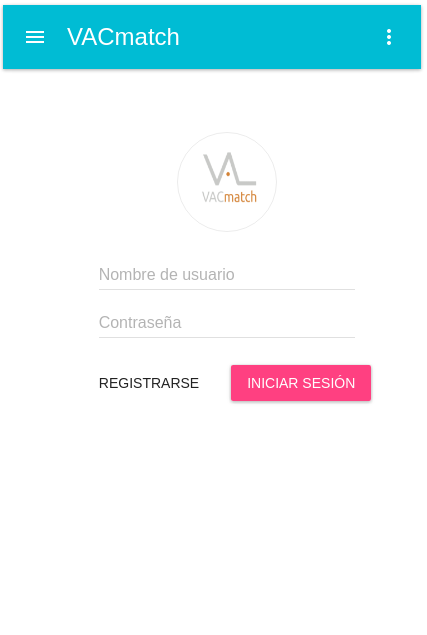
\includegraphics[width=0.4\textwidth]{./img/demo/6_login.png}
        \caption{Vista de inicio de sesión.}
        \label{fig:design:login}
        \end{center}
      \end{figure}

    \subsection{Listado de actas}
    Nesta sección podemos ver a lista de actas que un árbitro ten 
asignadas na Figura~\ref{fig:design:listreports}, divididas en dúas pestanas, 
por un lado as de próximos partidos a 
arbitrar e por outro aquelas nas que o encontro xa rematóu e que non é habitual 
que sexan accedidas.

      \begin{figure}[h!]
        \begin{center}
        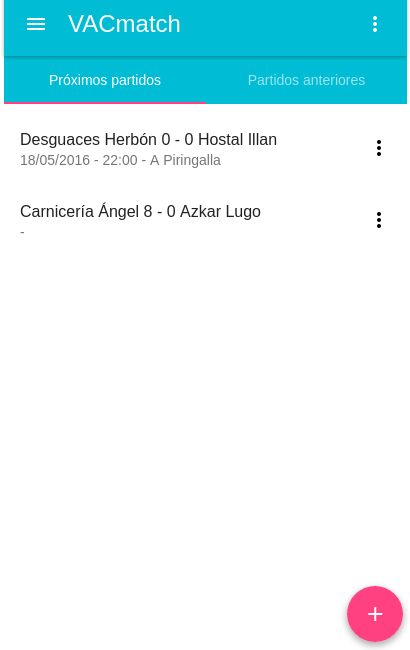
\includegraphics[width=0.4\textwidth]{./img/demo/7_reportlist.png}
        \caption{Listado de actas.}
        \label{fig:design:listreports}
        \end{center}
      \end{figure}

    Cada un dos elementos permítenos modificar a información 
básica da acta, tanto o nome dos equipos como o lugar de celebración ou a data 
por se é preciso edita ditos datos, permitindo do mesmo xeito eliminar a acta e 
tódolos elementos que a compoñen.

    Ademais, esta páxina danos a opción de engadir unha nova acta se é preciso, 
unha funcionalidade imprescindible xa que por múltiples razóns 
poderíase dar o caso de que a aplicación de un árbitro non sincronice as súas 
actas coas existentes na base 
de datos da federación, polo que o árbitro debe poder crear un acta baleira de 
xeito manual incluso sen ter conexión a internet.

    \subsection{Acta}
    Esta é a parte central da aplicación, con total seguridade será o lugar 
onde os usuarios pasarán a gran maioría do seu tempo de uso da aplicación xa 
que é o punto central do desenvolvemento dun partido.

    A acta dun encontro deportivo é un elemento con gran cantidade de 
información e que pode ser visualizada sen apenas esforzo xa que se atopa 
toda representada únicamente en unha folla de papel.

    É por iso que dende o primeiro momento se tiña claro que había que tratar 
de manter esa sinxeleza de uso pero, evidentemente, era imposible acceder a 
toda esa información en un só golpe de vista dentro de un soporte de un tamaño 
tan pequeno como é un teléfono móbil.

    Entón o enfoque foi un pouco diferente e tratouse de facer que o proceso de 
cubrir un acta resultase o máis interactivo posible, mostrando na pantalla 
central únicamente a información indispensable para o árbitro que está a 
cubrila.

    O deseño final pódese ver na Figura~\ref{fig:design:showreport} na que se 
mostran os seguintes campos:
    \begin{itemize}
     \item Os nomes dos equipos que están a competir con un enlace para ver os 
seus xogadores.
     \item Dóus campos de resultados.
     \item Un cronómetro.
     \item Un botón para comezar o encontro e xestionar o cronómetro unha vez 
comezou.
     \item Un botón de edición
     \item Un botón para mostrar os eventos que 
ocorreron.
     \item Botóns para engadir un dos diversos eventos que poden ser utilizados 
para este encontro
    \end{itemize}

    \begin{figure}[h!]
      \begin{center}
      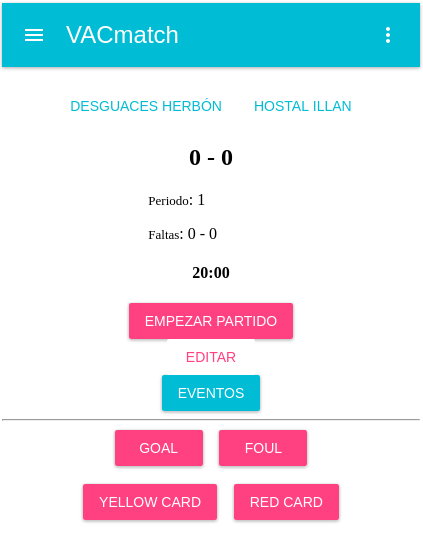
\includegraphics[width=0.5\textwidth]{./img/demo/8_report.png}
      \caption{Vista principal de un acta.}
      \label{fig:design:showreport}
      \end{center}
    \end{figure}

      \subsubsection{Convocar xogadores}
      Nas accións habituais que debe realizar un árbitro, o 
primeiro paso é cubrir no papel os nomes dos xogadores que se atopan presentes 
no encontro coas fichas identificativas que cada un de eles aporta.

      Como o obxectivo é eliminar o papel e simplificar o traballo do árbitro 
e da federación, a acta do encontro contén tódolos xogadores que 
se atopan inscritos no equipo correspondente coa sua foto como se pode ver na 
Figura~\ref{fig:design:callplayers}, polo que xa non son 
precisas as fichas en papel de cada un de eles e o árbitro non ten que escribir 
os nomes dos integrantes dos equipos, se non que únicamente debe seleccionar 
cales de eles se atopan no campo.

    \begin{figure}[h!]
      \begin{center}
      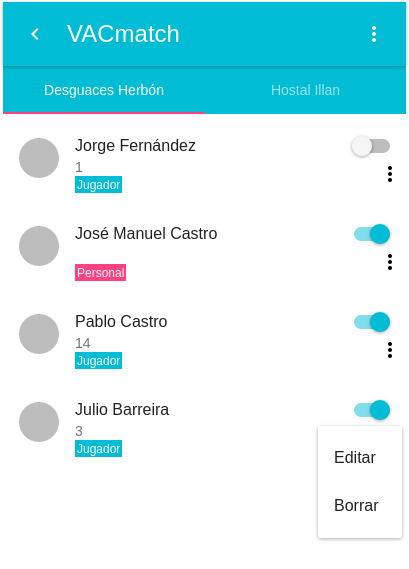
\includegraphics[width=0.5\textwidth]{./img/demo/9_calllist.png}
      \caption{Seleccionar xogadores presentes no encontro.}
      \label{fig:design:callplayers}
      \end{center}
    \end{figure}

      Tamén ten a posibilidade de editar o dorsal do xogador para este encontro 
en concreto xa que en algunhas competicións é habitual que os xogadores cambien 
de camiseta segundo o partido.

      Por último existe a opción de engadir un novo xogador de xeito 
manual, útil para o caso no que o árbitro teña que crear un acta manualmente ou 
para cando un novo xogador é engadido a un clube pero non é dado de alta na 
aplicación a tempo, e se o árbitro accede, este pode ser engadido a acta de 
xeito manual e competir sen problemas

      \subsubsection{Inicio e fin do partido}
      O seguinte paso á hora de xestionar a acta dun encontro é indicar cando 
comeza o mesmo, para isto o usuario dispón de un botón que só se mostra cando 
non comezou aínda dito partido e que se encarga de introducir un evento de 
comezo.

      No momento en que se comece o partido, atoparase dispoñible o botón 
que permite arrancar e deter o \textbf{cronómetro}, co fin de poder xestionar o 
encontro de xeito interactivo e que tódolos eventos introducidos leven 
incorporado o momento no que se produciron.

      Non é obrigatorio utilizar o cronómetro polo que os eventos poden ser 
engadidos en calquera momento e non se almacenará o minuto no que se produciron.

      Do mesmo xeito, pódese engadir un evento de fin de encontro nunha das 
opcións desplegables do menú superior dereito e que redirixirá ao árbitro a 
páxina de asinado de acta.

    \subsection{Finalización do encontro}
    Cando un árbitro decide rematar un encontro, accederá a esta última vista 
da aplicación que podemos ver na Figura~\ref{fig:design:endmatch} onde 
poderá engadir un texto coa información de posibles 
\textbf{incidencias} que ocorreran durante o encontro e que deben ser postas en 
coñecemento da federación, como algún tipo de agresión ou o motivo polo que un 
partido tivo que ser finalizado antes de tempo.

    \begin{figure}[h!]
      \begin{center}
      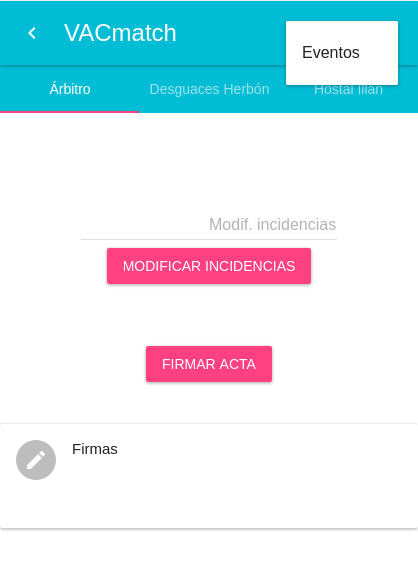
\includegraphics[width=0.5\textwidth]{./img/demo/10_endmatch.png}
      \caption{Fin de encontro.}
      \label{fig:design:endmatch}
      \end{center}
    \end{figure}

    Dende o menú superior dereito pódese acceder directamente aos eventos que 
ocorreron durante o partido. Isto resulta útil para mostrarlle as persoas que 
asinan a acta toda a información da acta para que poidan confirmar que 
realmente os eventos gardados na mesma, son certos.

    A vista ten varias pestanas, unha para o árbitro e outra para cada un dos 
equipos, onde poderán asinar a acta tantas persoas como sexa preciso.

    Unha vez se faga click no botón de asinar de algunha das pestanas, 
mostrarase unha listaxe coas persoas que poden asinar de cada equipo ou do 
equipo arbitral como podemos ver na Figura~\ref{fig:design:signreport}.

    Para realizar a sinatura, a persoa debe dispoñer de conta creada na base de 
datos da federación na que debeu de indicar previamente código PIN que lle 
permitirá asinar a acta.

    No caso de xogadores creados manualmente dende a propia aplicación móbil, 
poderase asinar a acta sen dispoñer de código PIN, deixando o oco baleiro.

    \begin{figure}[h!]
      \begin{center}
      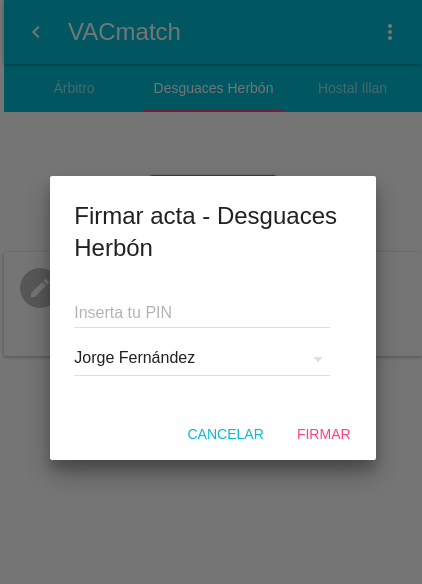
\includegraphics[width=0.5\textwidth]{./img/demo/11_sign.png}
      \caption{Sinatura de un acta.}
      \label{fig:design:signreport}
      \end{center}
    \end{figure}

    \subsection{Modificación de estilos}
    A xestión de estilos na aplicación varía de xeito considerable fronte ás 
aplicacións web habituais polo que é importante facer unha pequena reseña.

    Certa parte da comunidade de React defende que o estilo das aplicacións 
web, que tradicionalmente se xestiona a través de follas CSS, debe mudar e 
pasar a realizarse directamente en Javascript.

    Os estilos son inxectados directamente no compoñente de xeito ``inline'' a 
través do atributo ``style'' de HTML\footnote{A diferencia da maneira 
tradicional na que os estilos se compoñen en clases CSS a través do atributo 
''class'' e pódense anidar unhas con outras de forma declarativa}, coa idea de 
acabar con diversos erros de deseño en CSS, algúns dos cales se comentan a 
continuación.

    O feito de que os estilos sexan código global accesible dende calquera 
parte das aplicacións tradicionais, fai que esta sexa pouco consistente ante os 
cambios, unha pequena modificación pode cambiar gran parte da aplicación e pode 
ser dificil de atopar dito cambio cando os proxectos adquiren un certo 
tamaño polo que a xestión de xeito máis localizado a través de variables 
Javascript, facilitaría este mantemento.

    A eliminación de código morto tamén é outra das vantaxes de utilizar 
Javascript para este propósito xa que, agora os estilos serán variables locales 
que os ``minifiers''\footnote{Programas que eliminan código e 
caracteres inecesarios como os espacios ou tabulacións} de Javascript 
eliminarán automáticamente.

    Por último tamén aporta unha total flexibilidade, dando incluso a 
posibilidade de tratar os estilos como parte do estado da aplicación e 
convertilos de este xeito, en totalmente dinámicos.

  \section{Multideporte}
  Un dos obxectivos iniciais era conseguir que a aplicación poidera adaptarse 
de xeito moi sinxelo a novos deportes, inicialmente comezaríase co fútbol pero 
todo o deseño debía estar orientado cara esta finalidade.

  \subsection{Deporte}
  Para iso creouse unha \lstinline{SportStore} que contén a información do 
deporte 
que a aplicación está xestionando actualmente, e que pode ser actualizado e 
cambiado por outro, de xeito moi sinxelo.

  Dende múltiples compoñentes como por exemplo o \lstinline{PersonList}, pódese 
obter o deporte actual que está almacenado na Store e as múltiples propiedades 
que o definen, como se pode ver na Figura~\ref{fig:design:strategy}.

    \begin{figure}[h!]
      \begin{center}
      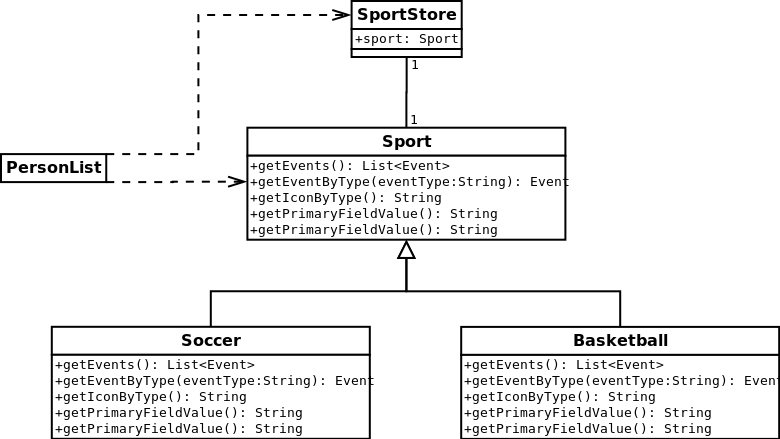
\includegraphics[width=0.8\textwidth]{./img/diagrams/sport_diagram.png}
      \caption{Patron estratexia para o deporte.}
      \label{fig:design:strategy}
      \end{center}
    \end{figure}

  Cada deporte debe extender a unha clase xenérica \lstinline{Sport} nun 
patrón Strategy\cite{book:patterns} que se pode observar na 
Figura~\ref{fig:design:strategy} e que define unha serie de métodos que tódolos 
deportes deben implementar, métodos que indican cómo se realizan certas accións 
sobre os datos en cada deporte.

  A continuación móstranse os parámetros que ten un \lstinline{Sport} 
actualmente:

  \begin{description}
   \item [Eventos] A lista de eventos que se poden realizar en ese deporte.
   \item [Evento por tipo] Permite recuperar un obxecto Evento a partir da 
clave do seu tipo.
   \item [Icono por tipo] Devolve o icono que identifica un Evento de un 
tipo para renderizalo en algunha parte da aplicación como a lista de eventos.
   \item [Campo primario] É unha función que calcula o resultado para 
almacenar no campo primario da acta en función da lista de eventos para ese 
encontro e de cada deporte. En fútbol devolve únicamente a suma de eventos de 
tipo gol.
   \item [Campo secundario] Similar ao campo anterior pero para introducir 
información no campo secundario da acta, no caso do fútbol, o campo secundario 
almacena as faltas do encontro e esta función devolve a suma de faltas que hay 
no partido.
  \end{description}

  Esta implementación fai que sexa tremendamente sinxelo engadir un novo 
deporte, básicamente deberíase crear unha nova clase que extendese os métodos 
correspondentes coa funcionalidade concreta de ese deporte.

  \subsection{Roles de usuarios}
  Actualmente a aplicación únicamente pode ser accedida por árbitros, usuarios 
con un rol concreto, pero resulta trivial engadir novos roles, como por exemplo 
o de administrador de unha federación, para que este poida crear tamén 
encontros dende a aplicación móbil.


  \subsection{Eventos}
  Do mesmo xeito, cada deporte ten os seus propios eventos polo que se definíu 
unha forma de engadir eventos novos de xeito sinxelo, co fin de que a 
incorporación de un novo deporte resultase o máis trivial posible.

  Actualmente podemos dividir os eventos en dous tipos:

  \begin{description}
    \item [De control] Son eventos xenéricos de xestión como cambiar de parte, 
ou comezar un encontro, que non é habitual que vaian a cambiar xa que son 
compartidos pola inmensa maioría de deportes.
    \item [De deporte] Son eventos concretos de cada deporte como engadir un gol 
ou unha tarxeta, a súa vez divídense en:
      \begin{description}
       \item [Evento] É un tipo de evento de deporte que únicamente permite ser 
engadido ou eliminado, non dispón de un comportamento especial.
       \item [Evento con causa] Este tipo de evento, engade tamén unha causa 
pola que se producíu, útil para indicar por exemplo a motivación que levou a 
un árbitro a expulsar a un xogador con unha tarxeta vermella.
         \item [Evento de puntuación] Tipo de evento que permite actualizar os 
campos de resultados, primario e secundario de forma automática ao ser engadido.
      \end{description}

  \end{description}

  Na Figura~\ref{fig:design:eventviewdiagram} podemos ver a relación existente 
entre a \lstinline{EventStore} que contén o estado dos eventos e os compoñentes 
da vista que os renderizan.

  Temos dous compoñentes de React para renderizar os eventos dentro da vista 
que lista tódolos eventos que suceden durante o partido, os compoñentes 
\lstinline{SportEvent} e \lstinline{ControlEvent}.

  Por outra banda temos tamén dous compoñentes de React que definen a vista que 
se ten que mostrar cando se desexe engadir un evento de este tipo dende a 
aplicación, son \lstinline{Event} e \lstinline{EventWithCause} que ademais 
mostrará unha lista de causas que poden ser engadidas ao evento.

    \begin{figure}[h!]
      \begin{center}
  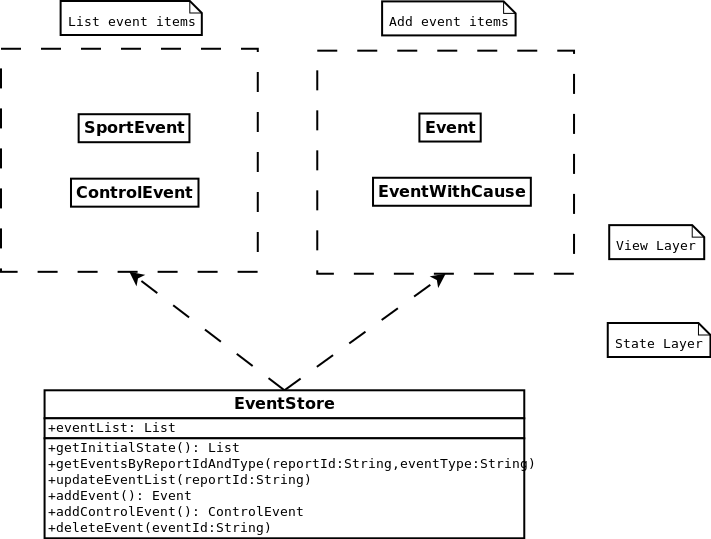
\includegraphics[width=0.8\textwidth]{./img/diagrams/events_view_diagram.png}
      \caption{Diagrama parcial da vista dos eventos.}
      \label{fig:design:eventviewdiagram}
      \end{center}
    \end{figure}


  En definitiva, para crear un novo evento débese definir unha clase Javascript 
coas propiedades do mesmo e que implemente ao \lstinline{SportEvent} como se 
pode ver na Figura~\ref{fig:design:eventsdiagram} a través dos exemplos de 
\lstinline{GoalEvent} ou \lstinline{FoulEvent}.

  Tamén é preciso engadir unha clase de React que defina as vistas que se 
mostrarán ao intentar engadir e listar un evento durante o encontro ou 
utilizar as xa definidas previamente que se poden ver na 
Figura~\ref{fig:design:eventviewdiagram}.

  Por último, como podemos observar de novo na 
Figura~\ref{fig:design:eventsdiagram}, débese engadir o evento creado 
anteriormente, dentro da lista de eventos que ten ese deporte, e que se atopan 
na clase que implementa dito deporte concreto.

    \begin{figure}[h!]
      \begin{center}
  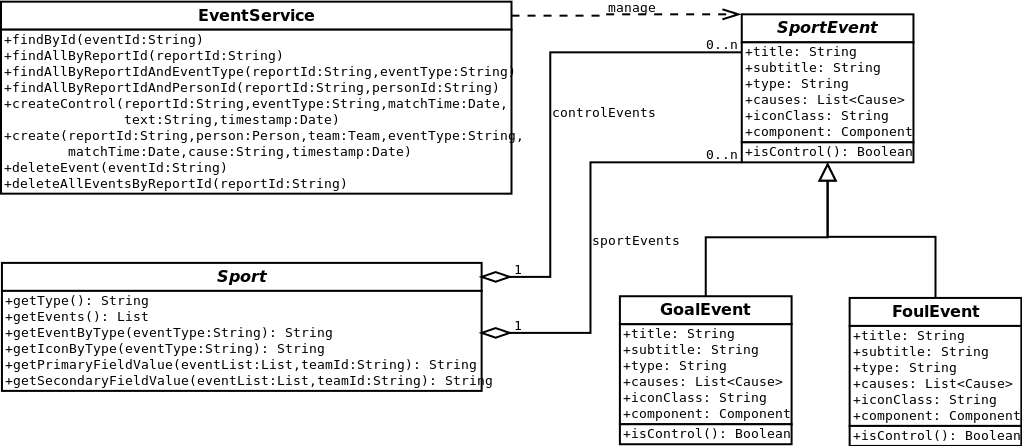
\includegraphics[width=\textwidth]{./img/diagrams/events_diagram.png}
      \caption{Diagrama de clases para a xestión de eventos.}
      \label{fig:design:eventsdiagram}
      \end{center}
    \end{figure}


  \section{Deseño da DB}
  VACmatch Mobile pensóuse inicialmente para ser integrado co sistema de 
xestión de competicións que estamos a desenvolver con VACmatch Web e que dispón 
dunha API de comunicacións que se atopa montada sobre unha base de datos 
relacional.

  É por iso que o modelo de datos inicial estaba plantexado para unha base de 
datos relacional e tivo que ser adaptado para utilizar unha non relacional 
orientada a documentos como é PouchDB.

  Prácticamente todas as entidades foron desnormalizadas para incluir 
información necesaria e en algún caso comprimíronse dúas entidades en unha soa 
como por exemplo en \lstinline{Call}\footnote{Convocatoria de un xogador para 
un partido en concreto} e \lstinline{Member} \footnote{Membro de un equipo} que 
foron unidas 
dentro de \lstinline{Person} como se pode ver na 
Figura~\ref{fig:design:persondbdiagram}

    \begin{figure}[h!]
      \begin{center}
      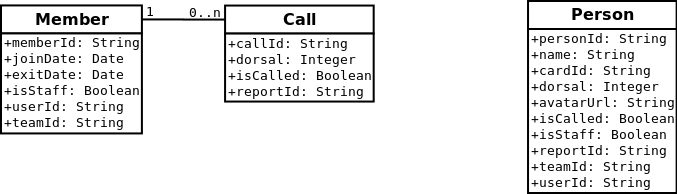
\includegraphics[width=0.8\textwidth]{./img/diagrams/person_diagram.png}
      \caption{Esquema base de datos de Person.}
      \label{fig:design:persondbdiagram}
      \end{center}
    \end{figure}

  \section{I18n}
  Para a xestión da internacionalización da aplicación utilizouse a librería 
React Intl que provee dunha serie de compoñentes de React e unha API sinxela 
para formatear datas, números e strings, incluindo pluralización e xestión de 
traducións.

  Esta librería dá a posibilidade de engadir un contexto aos textos que se 
internacionalizan, o cal facilita a labor do tradutor que se encargue de 
engadir ou modificar un idioma, proporcionándolle unha información extra sobre 
o texto que debe traducir.

  Únicamente é preciso definir os compoñentes cos seus correspondentes 
atributos como se mostra no Fragmento de código~\ref{fig:design:i18n} e a 
propia ferramenta xenera 
ficheiros \emph{.json} seguindo o esquema de carpetas e ficheiros da aplicación 
con toda a información recopilada.

    \lstset{}
     \begin{lstlisting}[caption=Exemplo de internacionalización 
na label de un botón., label=fig:design:i18n]
<RaisedButton label={
    <FormattedMessage
        id='report.show.events'
        description='Events button'
        defaultMessage='Events'/>
} secondary={true} style={style.button}/>
    \end{lstlisting}

  Do mesmo xeito, a librería permite facer internacionalización de xeito 
programático sen utilizar compoñentes de React, a través de unha serie de 
funcións de Javascript.

  Por último, é preciso realizar as traduccións aos diferentes idiomas, cada 
unha en un ficheiro de Javascript diferente, seguindo un formateado de 
pares cadea/valor.

  \section{Inxección de dependencias}
  Durante o realización do proxecto xurdíu problema entre os servizos xa que 
moitos precisan dos outros para realizar comprobacións de forma circular.

  A existencia de estas dependencias circulares leva a que sexa imposible de
determinar a relación entre eles polo que é preciso deseñar un pequeno sistema 
de inxección de dependencias que permite solventar esta problemática.

  A solución escollida finalmente consiste en crear unha factoría seguindo o 
patrón Singleton\cite{book:patterns} que se encarga de crear un obxecto para 
cada servizo e a continuación inxéctanse uns dentro dos outros.

  Cada vez que se chama a factoría para recuperar un servizo, esta
devolve o servizo coas súas dependencias inxectadas no seu interior polo que 
resolvemos o problema de xeito sinxelo.

  Na Figura~\ref{fig:design:dependency} pódese ver parcialmente o código que 
implementa a factoría que se encarga de crear os servizos e devolvelos cando é 
preciso.

    \lstset{}
    \begin{lstlisting}[caption=Fragmento da ServiceFactory., 
label=fig:design:dependency]
let ServiceFactory = {
  isInitialized: false,
  _servicesList: new Map(),

  constructor () {
    this._personService = new PersonService()
    this._reportService = new ReportService()
    this._refereeService = new RefereeService()
    // Without dependencies
    this._teamService = new TeamService()
    // Inject dependencies
    this._eventService.ReportService = this._reportService
    this._eventService.PersonService = this._personService
    this._eventService.TeamService = this._teamService
    ...
    // Add services to the exposed list
    this._servicesList.set('ReportService', this._reportService)
    this._servicesList.set('PersonService', this._personService)
    this._servicesList.set('TeamService', this._teamService)
    this.isInitialized = true
  },

  getService  (type) {
    if (!this.isInitialized) {
      this.constructor()
    }
    let service = this._servicesList.get(type)
    if (!service) {
      console.log('Error getting ', type, ' service')
    }
    return service
  }

}
    \end{lstlisting}

  Cómpre tamén comentar as dificultades que implica a inxección de dependencias 
ao realizar testing unitario xa que non se poden aproveitar as funcionalidades 
que aporta Jest, o framework de testing, que habitualmente permite automatizar 
a creación de mocks e, en este caso, obríganos a crear manualmente os mocks dos 
servizos e inxectalos dentro da clase a testear.

  \section{Testing e Integración continua}
  O testing é unha parte fundamental nun proxecto e concretamente nun proxecto 
de software libre no que a comunidade pode colaborar e onde poden 
participar persoas sen un coñecemento moi profundo da aplicación, polo que se 
fai totalmente imprescindible garantizar que calquera cambio non rompa a 
integridade da mesma.

    \subsection{TDD e BDD}
  Neste proxecto seguironse diversas prácticas de Test Driven Development 
(TDD)\cite{book:cleancode} e Behaviour Driven Development 
(BDD)\cite{book:cucumber} comezando por unha definición das 
diversas tarefas do proxecto como tests de aceptación das funcionalidades e 
rematando pola realización de tests unitarios.

      \paragraph{Tests de aceptación} Estos tests son destinados a determinar 
se foron cumplidos os requisitos dunha certa funcionalidade, sempre 
centrándose na parte funcional e alonxándose dos detalles de implementación.

      Para isto utilízanse unha linguaxe simple de dominio co fin de definir os 
requisitos funcionais, en este proxecto baseámonos no seguinte:

        \begin{description}
         \item [Como ....] afectado ou realizador da funcionalidade.
         \item [Quero ...] acción a realizar.
         \item [Cando ...] momento ou caso no que debe realizarse.
        \end{description}

        Un exemplo de test de aceptación:

        \emph{Como árbitro quero que o resultado se actualice automáticamente 
ao engadir un novo gol}.

      \paragraph{Tests unitarios} Estos tests céntranse en comprobar o 
funcionamento de xeito illado dos diversos sistemas e facendo fincapé en que 
cada proba sexa un caso totalmente independente do resto.

      En este proxecto crearonse tests unitarios centrados nos servizos da 
aplicación, que son os elementos máis importantes da mesma xa que son os que 
definen a lóxica de negocio.

      Para a realización de este tipo de tests é fundamental a utilización de 
mocks, obxectos que imitan o comportamento de obxectos reais de xeito 
controlado e que permiten simular o comportamento dos obxectos dependentes.

      Isto é fundamental para asegurar o illamento da funcionalidade e eliminar 
a dependencia de outros elementos a hora de realizar as probas unitarias.

    \subsection{Jest}
    É unha librería para realización de testing automático en aplicacións 
ReactJS que facilita automatizar a creación de mocks ou executar os tests con 
unha implementación falsa do DOM\footnote{Modelo en Obxectos para a 
Representación de Documentos}.

    No Fragmento de código~\ref{fig:design:test6} pódese observar un test 
de exemplo do módulo de eventos e os diversos compoñentes que o forman. 

    Inicialmente defínese dentro da sección \lstinline{describe} unha 
''historia de usuario`` que contén a información xeral sobre o caso de uso, 
dentro da cal pódense realizar diversos tests, no exemplo que vemos, o caso de 
uso é ''Crear un evento deportivo''.

    \lstset{}
    \begin{lstlisting}[caption=Definición de unha historia de usuario en Jest., 
label=fig:design:test1]
describe('create Sport Event', function () {
...
    \end{lstlisting}

    Dentro do caso de uso vemos un bloque \lstinline{beforeEach} que permite 
inicializar variables para cada novo test que se realice, eliminando de este 
xeito a dependencia entre os tests que as utilizan.

    Dentro do bloque \lstinline{describe} defínense os diversos tests desta 
historia de usuario, concretamente dentro dos bloques \lstinline{it}.

    \lstset{}
    \begin{lstlisting}[caption=Definición de un test en Jest., 
label=fig:design:test2]
it('Create a new Sport Event with valid parameters', function () {
...
    \end{lstlisting}

    Como comentábamos anteriormente, ao realizar tests unitarios é habitual a 
utilización de obxectos mock que imitan a funcionalidade de outros.
    En Jest todos os obxectos son mocks e non é preciso definilos todos así.
Cambiando un pouco a forma de traballar habitualmente, aquí débese definir ao 
comezo do ficheiro aqueles que non van a ser mockeados a través da sentencia 
definida no Fragmento de Código~\ref{fig:design:test3}.

    \lstset{}
    \begin{lstlisting}[caption=Sentencia para indicar que non se creen un 
mock., label=fig:design:test3]
jest.dontMock('../../src/app/models/report/status/StartedStatus')
    \end{lstlisting}

    Tamén é habitual querer darlle un comportamento por defecto aos mocks que 
se utilizan, por exemplo no Fragmento de Código~\ref{fig:design:test4} estamos 
facendo que cando se chame a función \lstinline{findById} do obxecto 
\lstinline{reportService}  co un só parámetro, o obxecto devolverá un callback 
cos parámetros indicados, neste caso unha Acta por defecto 
(\lstinline{defaultReport}) e un valor nulo como segundo parámetro.

    \lstset{}
    \begin{lstlisting}[caption=Sentencia para asignar comportamento a un mock., 
label=fig:design:test4]
spyOn(reportService, 'findById').andCallFake(function (anyReportId, callback){
  callback(defaultReport, null)
})
    \end{lstlisting}

    Unha vez definido o comportamento que queremos que teñan os mocks, debemos 
chamar ao método real do obxecto que estamos testeando e así teremos totalmente 
illado o comportamento de dito método.

    Finalmente utilizamos a cláusula \lstinline{expect} para indicar 
resultados esperados, no caso de exemplo que mostramos a continuación, estamos 
a indicar que a chamada ao método \lstinline{findById} de 
\lstinline{reportService} foi realizada. Tamén é posible indicar valores que 
debe devolver, negacións ou outras validacións incluso máis complexas.

    \lstset{}
    \begin{lstlisting}[caption=Sentencia para comprobar a execución de un 
test., label=fig:design:test5]
expect(reportService.findById).toHaveBeenCalled()
    \end{lstlisting}

    A continuación mostramos o caso de test anterior completo a modo de exemplo.

    \lstset{}
    \begin{lstlisting}[caption=Exemplo de test no módulo de eventos 
utilizando Jest., label=fig:design:test6]
describe('create Sport Event', function () {
  beforeEach(function () {
    defaultPerson = new Person(null, '', '', '', '', false, false, '', '',   '')
    defaultTeam = new Team(null, 'Team name')
    defaultReport = new Report(null, '', '', ReportStatus.READY, 
      defaultTeam, defaultTeam, [])
    defaultEvent = new EventElements.Event('event', '1', defaultPerson, 
      defaultTeam, 'goal', 1, 'cause', 1)
    reportService = new ReportService(jasmine.createSpy('PersonService'), 
      jasmine.createSpy('TeamService'), jasmine.createSpy('EventService'), 
      jasmine.createSpy('SignService'))
    personService = new PersonService(jasmine.createSpy('ReportService'), 
      jasmine.createSpy('TeamService'), jasmine.createSpy('AuthService'))
    teamService = new TeamService()
    eventService = new EventService(reportService, personService, 
      teamService)
  })

  it('Create a new Sport Event with valid parameters', function () {
    spyOn(reportService, 'findById').andCallFake(function(anyReportId,callback){
        callback(defaultReport, null)
      })

    spyOn(personService, 'findByPersonIdReportIdAndTeamId').andCallFake(function 
      (anyPersonId, anyReportId, anyTeamId, callback) {
        callback(defaultPerson, null)
      })

    spyOn(teamService, 'findById').andCallFake(function (anyTeamId, callback) {
      callback(defaultTeam, null)
    })

    spyOn(EventDao, 'create').andCallFake(function (reportId, person, team, 
      eventType, matchTime, cause, timestamp, callback) {
        callback(defaultEvent, null)
      })

    eventService.create(defaultEvent.reportId, defaultEvent.person, 
      defaultEvent.team, defaultEvent.type, defaultEvent.matchTime, 
      defaultEvent.text, defaultEvent.timestamp,
      (event, err) => {
        expect(event).toEqual(defaultEvent)
        expect(event).not.toBe(null)
        expect(err).toBe(null)
      })

    expect(reportService.findById).toHaveBeenCalled()
    expect(personService.findByPersonIdReportIdAndTeamId).toHaveBeenCalled()
    expect(teamService.findById).toHaveBeenCalled()
    expect(EventDao.create).toHaveBeenCalled()
  })})

  \end{lstlisting}

    \subsection{Travis CI}
    A medida que a aplicación foi medrando, xurdíu a necesidade de simplificar 
traballos como a búsqueda de erros ou o mantemento da aplicación, buscando 
garantir que se mantén a integridade da mesma en todo momento e non se 
introducen erros polo que se decidíu engadir tests unitarios na aplicación.

    Da mesma maneira lanzóuse unha primeira vesión estable do proxecto polo 
que tamén se decidíu engadir un sistema de integración continua ao mesmo co 
fin de garantizar que a aplicación xerada na rama de producción é funcional, 
compila en todo momento e pasa tódolos tests.

    Para isto utilizóuse Travis CI como sistema integración para o que se 
engadíu un ficheiro \emph{``.travis.yml''} no que se lle indican diversos 
parámetros de configuración, como as versións de Javascript coas que debe poñer 
a proba o funcionamento do programa, os scripts a executar para instalar 
dependencias e para executar o programa, as ramas de desenvolvemento sobre as 
que debe actuar, no noso caso \lstinline{master} e \lstinline{development} ou 
as notificacións 
que debe enviar ao finalizar un traballo, por exemplo a través de correo 
electrónico ou utilizando un servizo de mensaxería instantánea como Slack.

    Nesta integración xurdíu un problema derivado do sistema de construcción 
utilizado no proxecto, Gulp, que nos axuda a automatizar tarefas como a 
compilación, a execución dos tests ou o deploy da aplicación, e derivado tamén 
do framework de tests, Jest.

    Cando este último se executaba a través de Gulp, non devolvía os 
erros ao resolver os tests como resultado dunha función, se non que o facía a 
través de un callback. É por iso polo que foi preciso engadir na tarefa 
''test`` definida en Gulp, o control de este caso para evitar falsos positivos 
na execución dos tests unitarios dende Travis.
